% Source of the figure chain-threads.pdf (layout of the construction: the chain and one thread).
% Compile with pdfLaTeX; the PDF is included in the manuscript at its natural size.
\documentclass[tikz,border=1pt]{standalone}
\usepackage[T1]{fontenc}
\usepackage{stix}
\pdfinfoomitdate=1 \pdftrailerid{} \pdfsuppressptexinfo=-1
\definecolor{threadred}{RGB}{200,40,40}
\begin{document}
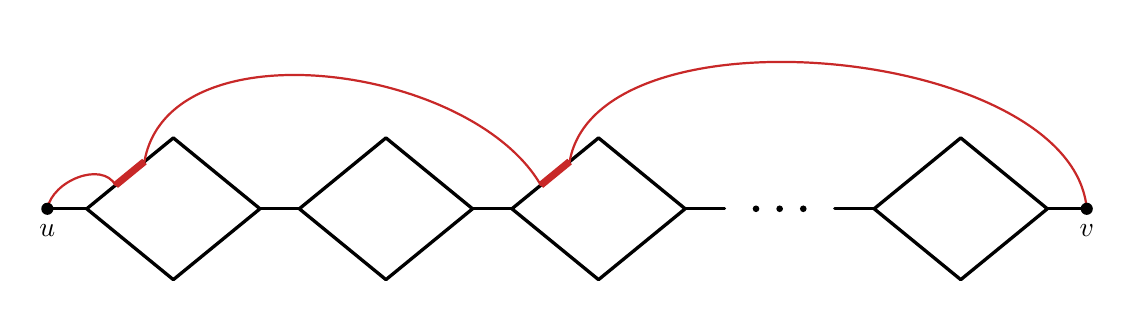
\begin{tikzpicture}[x=1cm, y=1cm,
    chain/.style={line width=1.2pt, line cap=round, line join=round},
    thread/.style={line width=0.8pt, line cap=round},
    crossing/.style={line width=2.6pt, line cap=butt},
    lead/.style={thread, densely dashed}]
  \useasboundingbox (0.15,-1.0) rectangle (13.85,2.3);
  % A chain link without a name: #1 = x-coordinate of its center.
  \newcommand{\chainlink}[1]{%
    \draw[chain] (#1-1.1,0) -- (#1,0.9) -- (#1+1.1,0) -- (#1,-0.9) -- cycle;}
  % A vertex with its name below: #1 = x-coordinate, #2 = name.
  \newcommand{\vertex}[2]{%
    \fill (#1,0) circle[radius=2.2pt];
    \node[below=2pt] at (#1,0) {#2};}

  \chainlink{2.0}
  \chainlink{4.7}
  \chainlink{7.4}
  \chainlink{12.0}
  \draw[chain] (0.4,0) -- (0.9,0)  (3.1,0) -- (3.6,0)  (5.8,0) -- (6.3,0)  (8.5,0) -- (9.0,0)
               (10.4,0) -- (10.9,0)  (13.1,0) -- (13.6,0);
  \foreach \x in {9.4,9.7,10.0} \fill (\x,0) circle[radius=1.2pt];

  % thread: from u through the first and the third chain link to v
  \draw[thread, threadred] (0.4,0) to[out=80, in=120] (1.267,0.3);
  \draw[thread, threadred] (1.633,0.6) to[out=80, in=120, looseness=0.9] (6.667,0.3);
  \draw[thread, threadred] (7.033,0.6) to[out=80, in=95, looseness=0.8] (13.6,0);
  \draw[crossing, threadred] (1.267,0.3) -- (1.633,0.6);
  \draw[crossing, threadred] (6.667,0.3) -- (7.033,0.6);
  \vertex{0.4}{$u$}
  \vertex{13.6}{$v$}
\end{tikzpicture}
\end{document}
